\chapter{学び}

\section{共通認識の重要さ}
本グループでは，プロダクトのテーマ決めから現在に至るまで，メンバー全員で共通認識を持つことを重要視してきた．伊藤恵教授から貸して頂いた書籍\wasyo{SCRUMMASTER THE BOOK 優れたスクラムマスターになるための極意――メタスキル，学習，心理，リーダーシップ}\cite{scrumm}に書かれていた通り，グループメンバー全員がプロダクトのターゲットや目的に対し共通認識を持つことは開発を進めるにあたって必要不可欠であるため，これらについて優先的に話し合ってきた．また，チームメンバーそれぞれの役割についても認識のずれが生じないよう全員で確認し合った．これによって，開発や中間発表の提出物作成を円滑に進めることができた．今後の開発においても，グループメンバー間で認識にずれがあった場合，プロダクトに支障をきたすため，細かなことでも，共通認識を持つことは重要であると考える．


\bunseki{鈴木利芳}

\section{議事録の重要さ}
本グループでは，何をどのように決定し，いつ何が決定されたかを後から確認できるよう議事録をとりながら活動を進めた．議事録は，決定した内容や過程だけでなく，決定に至るまでの思考や発言も記録する必要があるため，多くの肉体的コストがかかるが，それを上回るメリットがあることを学んだ．特に，報告書やポスター，発表スライドの作成の際は，議事録を見直すことで作業をスムーズに進めることができ，メリットを享受することができた．また，議事録に，次週の活動方針や次週までに達成したい目標を記録することで，グループメンバーがそれぞれ何をやらなければいけないのかが明確になった．これにより，開発をスムーズに行えるだけでなく，グループメンバーの共通認識を明確にすることができた．議事録は，これまでの開発を振り返り，これからの活動方針を決定するためにも，必要不可欠なものであると考えられる．
\begin{figure}[H]
    \centering
    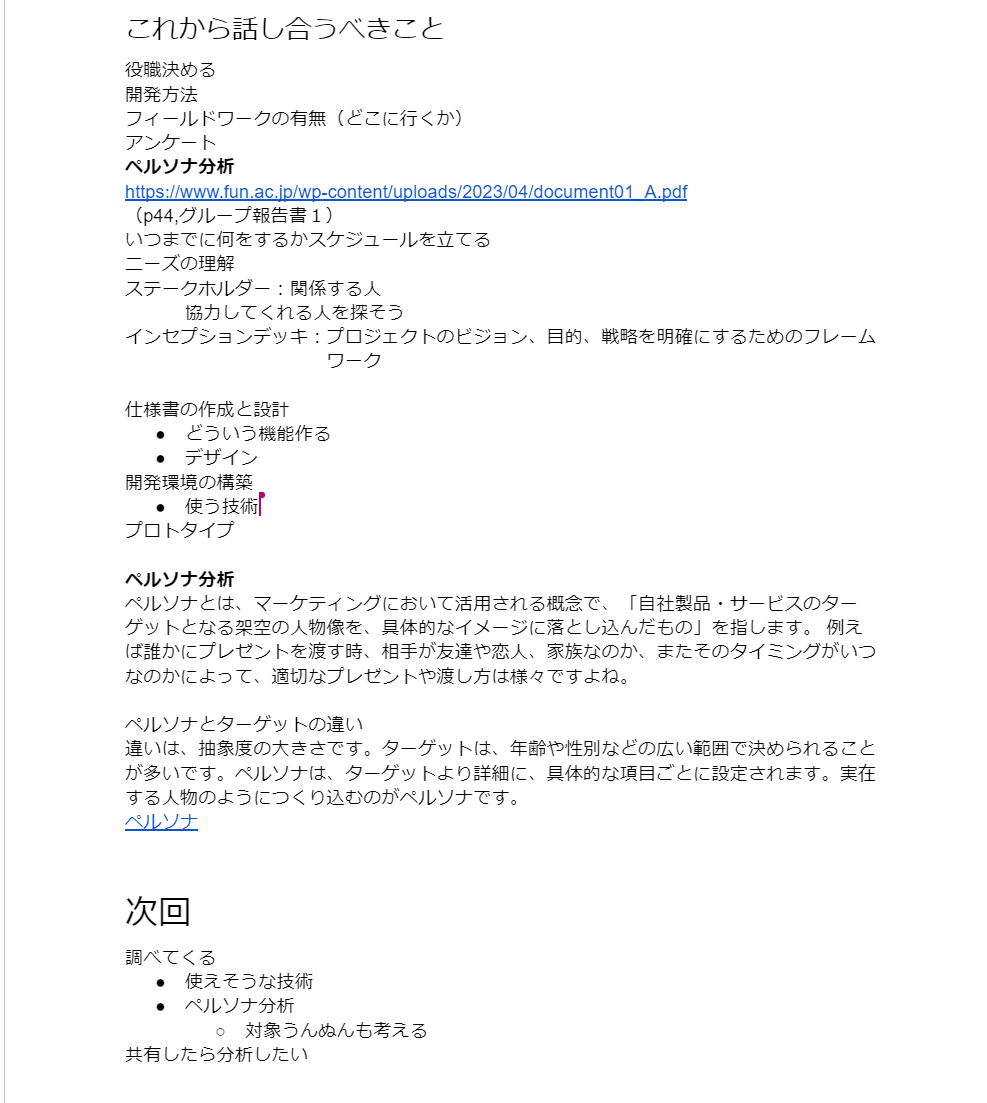
\includegraphics[height=16cm]{images/5.2_giziroku.png}
    \caption{実際の議事録の様子（一部を抜粋）}
    \label{fig:giziroku}
\end{figure}
\bunseki{鈴木利芳}

\section{コミュニケーションツール}
%各人の担当課題の成果について，成果によってどのように上述した課題が解決されたか， 要求された役割は果たせたか，残された問題点はあるかを記述する．

\subsection{Discord}
プロジェクト時間外の活動で話し合いを行うためにDiscord\footnote{https://discord.com}を利用した．Discordとは，アメリカ発祥のチャットサービスである．Discordはオンラインゲームをしながら，世界中の人々とコミュニケーションをとるために生まれたサービスであるが，最近では，さまざまなコミュニティで利用されている．私達は，遠隔でも作業を効率よく進めるためにボイスチャットや画面共有機能を使用した．ボイスチャットや画面共有を使うことで，現在行っている作業の何に困っているかが明確になったことや，すぐに意見を求めたり意見を言ったりすることができた．
\bunseki{南川虎之介}

\subsection{Slack}
プロジェクト活動の進捗報告や連絡事項などを補助するツールとしてSlack\footnote{https://slack.com}を利用した．Slackとは，チャンネルベースで行われるビジネス用のメッセージングアプリである．一般的にSlackはグループコミュニケーションツールとして使われている．このツールを使うことで，メンバーが1つの場所に集まり，グループが一体となって働くことができた．
\bunseki{齊藤輝}

\subsection{ホワイトボード}
グループ活動で話し合うときは，主にホワイトボードを用いて活動していた．ホワイトボードを使う場面のほとんどはブレインストーミングを行うときである．グループメンバーの意見やホワイトボードにすべて書くことで思考を発散させた．これにより，プロダクト案プロダクトの対象者などを明確にする一助になったため，何かに行き詰まって困ったときは，ホワイトボードでブレインストーミングを行うことがいいということを学んだ．
\bunseki{斎藤輝}

\section{Figma}
Figma\footnote{https://www.figma.com}とは，ブラウザ上で動作し，デザインの作成，共有を簡単に行うことができるツールである．複数人同時での編集や閲覧が可能であるため，本開発で使用することにした．本開発では，プロダクトのUIデザインやプロトタイプの作成に使用した．
\bunseki{鈴木利芳}

\section{Git/GitHub}
Git\footnote{https://git-scm.com}とは，ソースコードの変更を保存，追跡するための分散型バージョン管理システムである．GitHub\footnote{https://github.com}とは，Gitを用いてクラウド上でバージョン管理をすることができるWebサービスである．複数のユーザーと共有し，共同作業を行うことができる．
\bunseki{南川虎之介}



